%===== Settings =====
\documentclass[10pt, conference, compsoc]{IEEEtran}

% input encoding
\usepackage[utf8]{inputenc}
\usepackage[english]{babel}

%create graphics
\usepackage{tikz}
\usetikzlibrary{shapes.geometric, arrows}

\tikzstyle{startstop} = [rectangle, rounded corners, minimum width=1cm, minimum height=1cm,text centered, draw=black, fill=red!30]
\tikzstyle{io} = [trapezium, trapezium left angle=70, trapezium right angle=110, minimum width=1cm, minimum height=1cm, text centered, draw=black, fill=blue!30]
\tikzstyle{process} = [rectangle, minimum width=1cm, minimum height=1cm, text centered, draw=black, fill=gray!30]
\tikzstyle{decision} = [diamond, minimum width=1cm, minimum height=1cm, text centered, draw=black, fill=green!30]
\tikzstyle{arrow} = [thick,->,>=stealth]


% PDF figures
%\usepackage[pdftex]{graphicx}
%\DeclareGraphicsExtensions{.pdf,.png,.jpg}
\usepackage{float}

% additional packages
\usepackage{url}

%acronyms
\usepackage[printonlyused,withpage]{acronym}
\section*{Acronyms}
\begin{acronym}[II4.0MM]
\acro{BAS}{Building Automation Systems}
\acro{BIM}{Building Information Modeling}
\acro{BMN}{St. Gallen Business Model Navigator}
\acro{BMS}{Building Management Systems}
\acro{CPS}{Cyber-Physical-Systems}
\acro{DIHK}{German chamber of Industry and Commerce}
\acro{DRA}{Digital Readiness Assessment}
\acro{DT}{Digital Transformation}
\acro{I4.0Init}{Industrie 4.0}
\acro{I4.0}{Industry 4.0}
\acro{II4.0MM}{Individual I4.0 Maturity Model}
\acro{IIC}{Industrial Internet Consortium}
\acro{ISIC}{International Standard Industrial Classification of All Economic Activities}
\acro{IoT}{Internet of Things}
\acro{KPI}{Key Performance Indicators}
\acro{PR}{pull request}
\acro{RAMI}{reference architecture model for Industry 4.0}
\acro{SME}{Small and medium-sized enterprise}
\acro{UN}{United Nations}
\acro{WEF}{World Economic Forum}
\end{acronym}
% set PDF version to 1.6
\pdfminorversion=6

% hyphenation
%\hyphenation{}


%citing author name inline
%not working without author information on every source in .bib file
\usepackage[numbers]{natbib}


%===== Document start =====
\begin{document}% max 10 pages,

%===== Title & stuff =====
\title{Industry 4.0 – towards an industry-centric viewpoint}

\author{
	\IEEEauthorblockN{Pascal Brokmeier (B.Sc.)}
	\IEEEauthorblockA{Universität zu Köln, Germany \\ Email: pbrokmei@smail.uni-koeln.de}
	\and
	\IEEEauthorblockN{Jonathan Ott (B.Sc.)}
	\IEEEauthorblockA{Universität zu Köln, Germany \\Email: jott01@smail.uni-koeln.de
	}
}

\maketitle

%===== Text Begin =====
\begin{abstract}% max 150 words
TO BE DETERMINED
\end{abstract}

%\begin{IEEEkeywords}
% a, b, c
%\end{IEEEkeywords}


\section{Introduction}\label{Introduction}
% what is Digital Transformation and why is it being proposed to happen
\ac{DT}, the \ac{IoT}, Smart Factories,
\ac{I4.0}. Many words describing a vague ex ante declared
\emph{revolution} of the economy that many scientists and professionals are discussing.
% Gartner prophesizes over 6 billion IoT devices in use by the end
%of 2016 with over 13 billion expected by 2020
%\cite{gartner-iot-number-devices}.
There is a big interest from the public and private sections with many big consulting companies offering services to their customers regarding strategy, implementations, project management and technological support.
\cite{westerman2011digital,mckinsey-nine-questions,bcg-dt,accenture-dt:2015}.
Nonprofit organizations and governments are also organizing initiatives and associations like the German governments \emph{\ac{I4.0Init}} \cite{i40-web} initiative or the \emph{\ac{IIC}} \cite{iic-web} based in the United States.
%- most are focused on 3-4 industries

However, most are focusing on a few core industries, not following a systematic approach of evaluating the effect of the impeding changes on all sections \cite{westerman2011digital, pwc2016survey}. 
%- many industries, although interesting, are left out or just touched in single, specialised articles
Many industries, e.g. construction, although interesting, are often left out or considered only in separate specialised sources \cite{rolandbergerBauwirtschaft:2016}. 
%- big initiatives by governments or corporate associations try to cover all industries but still, they are missing some
Even the nation wide initiative \acl{I4.0Init} is specialised and focuses only on a subset of the whole variety of sections \cite{umsetzungsstrategie:2015}. 
%- a formal overview of all sections and a mapping of guidelines for each is needed to get an overview of the true cross-section-spanning nature of the \ac{DT}

A complete list of all sections has been developed by the United Nations in the \ac{ISIC}\cite{ISIC:2008}. A formal overview including all sections defined in this empirically based paper can ensure the complete coverage of all sections regarding their potential for \ac{I4.0} and \ac{DT}. The research question therefore is the following:
%- RQ: What generic and specialised guidelines exist for all sections regarding the implementation of an \acf{I4.0} strategy?

\emph{What guidelines exist for each section regarding the implementation of an \acf{I4.0} strategy?}


This question consists of three key aspects that will be put together to create a structured strategic process recommendation:
\begin{itemize}
    \item \textbf{Find frameworks}, initiatives and consortia adequate for a wide variety of businesses offering a holistic view on \ac{I4.0} and \ac{DT}
    \item \textbf{Evaluate each section} to find suiting frameworks
    \item Individualize recommendations based on a \textbf{companies state of digitalization}.
\end{itemize}

The expected result is a systematic overview of all sections and frameworks that can be used as guidelines for developing \ac{I4.0} strategies independent of a companies section or size. 
% what implications are foreseen and what does this mean for organizations
%====SNIPPET TAKE ====
%A wide range of industries are affected \cite{westerman2011digital,iic-web}. Companies like Uber and Tesla are intentionally pushing into the market of autonomous driving \cite{uber-autonomous,tesla-autonomous-blog}, a facet of the digital transformation, but virtually any company can get involved, even if they did not intend to as a recent case of DDOS cyber attacks showed which disabled big parts of the U.S. internet connectivity and left thousands of companies out of touch with their customers. The attackers used a large number of hacked IP security cameras which reminded organizations about a core challenge, IT security \cite{forbes-ddos-cameras}, as well as the fact that any company that is currently doing business will have to adapt to the digital transformation of our economy.

% What guidelines are already existing

%====SNIPPET TAKE ====
%With a variety of organizations and businesses showing interest in the development, the need for standardization and common structures becomes inherent to increase compatibility, avoid duplicate efforts and increase positive network effects. The German \ac{I4.0} initiative for example developed a \emph{\ac{RAMI}} for companies to use as a base of classifying standards and coordinating efforts. 
%who is left out ?
%This initiative however has a strong focus on manufacturing industries, a focus that has been apparent throughout our literature review. Other industries such as "Agriculture, Construction, Financial Services or Wholesale and retail trade" are seldom the focus \cite{bauer2015industrie,barometer:2016}. 

%====SNIPPET TAKE ====
%While the market is buzzing and everyone is talking about the expected changes, strategic business decisions, especially those that commit significant resources and create technological or economical dependencies, should be evaluated thoroughly to ensure success of the business.

%Due to the variety of frameworks, white papers and consulting offers found in our research as well as the imprecise use of many terms and concepts by most sources we want to create a guideline for managers intending to ready their organization for the \acl{I4.0}, independent of their industry along the following question:

%research question
%\emph{How can organizations strategically approach Industry 4.0, specific to their organizational environment and industry, integrating both their own previous efforts as well as global initiatives and frameworks to receive individual implementation recommendations.}




%JO
%TODO DONE 1) "many professionals are buzzing about" finde ich noch nicht gut formuliert. Vorschlag: "many scientists and professionals are discussing about" 
%TODO DONE 2) Japan IVI ausschließen? Haben wir ja nicht weiter betrachtet. 

\subsection{Methodology}

To answer our research question we approached the three mentioned aspects of the question systematically. First we performed a literature review, looking for frameworks, guidelines and other forms of guidance for companies looking to ready themselves for the \ac{I4.0}. 
%TODO how many did we look at? and which did we choose? literature review statistics
We selected those that had a holistic view on many sections or that covered those sections that were usually left out by most others. Initiatives that involve a large amount of global enterprises were considered more promising than frameworks developed by a single business or research team, simply because they have a bigger global influence. From now on we will call these resources simply "framework" as they represent such a structure.

Secondly, to ensure considering all relevant industries in our evaluation, we used the \ac{ISIC} developed by the United Nations to start our filtering of frameworks, mapping the aggregated, globally defined 11 sections of industries \cite{ISIC:2008} to those that were found in the literature review. Where possible, we match an industry to a framework that is directly applicable, otherwise evaluating whether a frameworks recommendations can be applied also to the industry that was not specifically mentioned in the literature reviewed. 

Finally we suggest an industry-focused, applicable model for businesses to rate themselves as well as their competition, so they can compare their current maturity state with a target state of digitalization. We focus on three categories: technology \& operations, business model and culture, as suggested by the \ac{WEF} whitepaper \cite{worldforumdigitalenterprise:2016}.


 				%1. Introduction
\subsection{Terminology}
In this subchapter some terms will be defined. This is important because of the mixed use of many different terms to describe similar concepts in both literature and colloquially by professionals.

\begin{itemize}

\item \textbf{Internet of Things:} Citing \citeauthor{iot-def:2016}, the \ac{IoT} is \emph{"the network of physical objects that contain embedded technology to communicate and sense or interact with their internal states or the external environment"}.
  
  
  \item \textbf{\acl{CPS}:} The term \ac{CPS} refers to the \emph{"tight conjoining of and coordination between computational and physical resources."}. They \emph{"far exceed those of today in terms of adaptability, autonomy, efficiency, functionality, reliability, safety, and usability"}. They are expected to \emph{"provide large-scale, distributed coordination (e.g., automated traffic control), [be] highly efficient (e.g., zero-net energy buildings), augment human capabilities, and enhance societal well being"}  \cite{cps:nsf:2011}
  
  \item \textbf{Cloud Computing} is a \emph{"model for enabling ubiquitous, convenient, on-demand network access to a shared pool of configurable computing resources that can be rapidly provisioned and released with minimal management effort or service provider interaction"}\cite{Mell:2011:SND:2206223}.
  
  \item \textbf{Digitalization:} \citeauthor{khan-digital:2016} simply calls it the \emph{"process of information conversion from the physical to the digital plane"}. Gartner however extends this by describing it as the \emph{"use of digital technologies to change a business model and provide new revenue and value-producing opportunities; it is the process of moving to a digital business"}. The term \emph{digitization} is sometimes used as a synonym to digitalization but we will stick to the former as suggested by \citeauthor{khan-digital:2016}.
  
  \item \textbf{Digital Transformation:} A term that is being described as \emph{"the use of technology to radically improve performance or reach of enterprises"}\cite{westerman2011digital} by the MIT Center for Digital Business can better be put in context by describing it as \emph{"the global accelerated process of technical adaptation by individuals, businesses, societies and nations, which comes as a result of digitalization"}\cite{bonnect2014leading,khan-digital:2016}.
  
  \item  \textbf{Industry 4.0:} Is derived from the German \emph{Industrie 4.0} and describes the German initiative with the same name. It is also sometimes used as a synonym for digitalization in the manufacturing sector \cite{McKinseydigitizationIndustrialSector:2015}, however mostly in the German speaking regions. We consider it as the \acl{DT} of the manufacturing sector.


  \item \textbf{Industry:} An industry is \emph{"defined as the set of all production units engaged primarily in the same or similar kinds of productive activity"}\cite{ISIC:2008}. This is important to differentiate from the German \emph{"Industrie"} which is largely equivalent to the more specific \emph{manufacturing industry}. We will, to avoid confusion with the term industry 4.0 and to follow a systematic approach, use the term 'section' to describe groups of industries. The term has a more abstract connotation and has also been used by \ac{UN} in \ac{ISIC}\cite{ISIC:2008}. 
%TODO !!!!!!! replace all 'industry' or 'sector' with 'section'

\end{itemize}

\ac{IoT}, \ac{I4.0}, \ac{CPS} and Cloud Computing can be considered initiators or enabling technolgies that lead to an increase of digitalization in business and society. This increased digitalization, which can be considered a continuous process, now causes a sudden surge in adaptation and investments by businesses and consumers alike into these technologies that have such wide effects on all aspects of society that it is considered a transformation or revolution \cite{Kagermann:2013}. 
Figure \ref{fig:terms} summarizes the different terms and their interrelation.

\begin{figure}[H]
\centering
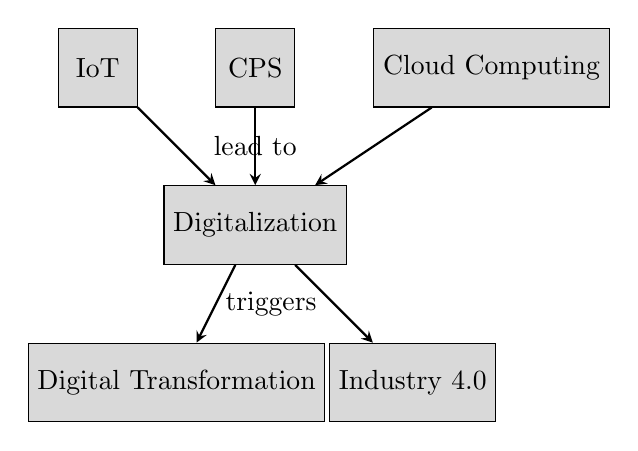
\begin{tikzpicture}[node distance=2cm]

%first row
\node (IoT) [process] {IoT};
\node (CPS) [process, right of=IoT, xshift=0cm] {CPS};
\node (CC) [process, right of=CPS, xshift=1cm] {Cloud Computing};
%second,third row
\node (D) [process, below of=CPS] {Digitalization};
\node (DT) [process, below of=D, xshift=-1cm] {Digital Transformation};
\node (I40) [process, right of=DT, xshift=1cm] {Industry 4.0};

%arrows
\draw [arrow] (IoT) -- (D);
\draw [arrow] (CPS) -- node {lead to}  (D);
\draw [arrow] (CC) -- (D);
\draw [arrow] (D) -- node [xshift=0.7cm]{triggers}(DT);
\draw [arrow] (D) -- (I40);


\end{tikzpicture}
\caption{Relation between terms} \label{fig:terms}
\end{figure}

%JO
%TODO 1) Framework als Begriff klarstellen? 2) Maturity Model mit aufnehmen sobald wir dieses festgelegt haben
 				%2. Terminology
\section{Methodology}

To answer our research question we approached the three mentioned aspects of the question systematically. First we performed a literature review, looking for frameworks, guidelines and other forms of guidance for companies looking to ready themselves for the \ac{I4.0}. We selected those that we deemed most promising based on a qualitative review. Initiatives that involve a large amount of global enterprises were considered more promising than frameworks developed by a single business or research team, simply because they have a bigger global influence. From now on we will call these resources simply "framework" as they represent such a structure.

Secondly, to ensure considering all industries in our evaluation, we used the \ac{ISIC} developed by the United Nations to start our filtering of frameworks, mapping the globally defined 21 sectors of industries \cite{ISIC:2008} to those that were found in the literature review. Where possible, we match an industry to a framework that is directly applicable, otherwise evaluating whether a frameworks recommendations can be applied also to the industry that was not specifically mentioned in the literature reviewed. 

Finally we used a model <FILL MODEL NAME @OTT> by <AUTHOR?> to challenge a business to rate itself regarding its "state of digitalization". Companies with little previous activity and a low grade					%3. methodology
\section{Components of a digital strategy}
To develop a strategy for responding to the impeding changes accompanying \ac{I4.0}, a business should first investigate what components this strategy is composed of. While the goal of an \ac{I4.0} strategy is apparent, as it is usually congruent with the general economic goals of the business itself, the implementation of this goal is dependent on three fields:

%We expect everyone to be familiar with the topic of digital transformation so we will refrain from describing estimates of future economic values that range from several hundred billion to a few trillion dollars total. %TODO citation
%We also assume most readers have heard the terms Internet of Things, Industry 4.0 or digital transformation. The argument for why businesses need to carefully evaluate how they implement their strategy and why they execute certain activities can be split into three categories:

\subsection{Technology}
The concept of digital transformation suggests that the entire business goes digital. It also implies that companies will have to adapt to a range of new technologies %TODO cite world http://reports.weforum.org/digital-transformation-of-industries/an-introduction-to-the-digital-transformation-of-industries-initiative/
 each of them potentially affecting an organizations core business. These technologies are not yet standardized nor established and some might be considered obsolete again in the near future. While businesses need to innovate to ensure they differentiate from their competitors, %source lecture Schrader? 
 they also need a stable core business to reduce risks. Open standards and technologies that have been widely accepted can offer these securities.
 % Instead of evaluating all these things by themselves, businesses should look towards existing organizations in the form of industry consortia and other non-profit structures to follow their guideline. By doing this, businesses can


%technology

\subsection{Business Models}
A popular term, disruption, describes what technology innovation does to markets. A new technology can lead to a complete overhaul of existing markets and it is usually accompanied by a different business model that catches existing market players off guard \cite{LucasJr200946}. \citeauthor{gassmann2013geschaeftsmodelle} suggest that a core challenge for businesses it not only to be a technological leader but also to develop a new business model that challenges existing market participants and helps a business to differentiate its product from the rest. 

\subsection{Culture}
\citeauthor{hammer:2015, LucasJr200946} argue a core task of preparation is the adaptation of the organizational culture to enable openness to innovation and adaption to new market environments. Businesses need to be "results-oriented", allow their employees to have the "freedom to increase innovation"\cite{hammer:2015} and avoid a culture that "promotes hierarchy and maintain[s] the status quo [because it] will be resistant to disruptive technologies"\cite{LucasJr200946}.
%business models
%culture
%disruption
 				%4. components digital strategy
\section{Background}
In the following chapter we will introduce some fundamental knowledge necessary to understanding the topic as well as our approach of developing recommendations for each section. We will first define a clear terminology that will be used in the remaining chapters. Afterwards, an adaptation of the recommendations given by the \ac{WEF} are described which we consider the core ingredients of a digital strategy \cite{worldforumdigitalenterprise:2016}. Finally, the most holistic frameworks, applicable to many sections, will be briefly introduced and described.

\subsection{Terminology}
In this subchapter some terms will be defined. This is important because of the mixed use of many different terms to describe similar concepts in both literature and colloquially by professionals.

\begin{itemize}

\item \textbf{Internet of Things:} Citing \citeauthor{iot-def:2016}, the \ac{IoT} is \emph{"the network of physical objects that contain embedded technology to communicate and sense or interact with their internal states or the external environment"}.
  
  
  \item \textbf{\acl{CPS}:} The term \ac{CPS} refers to the \emph{"tight conjoining of and coordination between computational and physical resources."}. They \emph{"far exceed those of today in terms of adaptability, autonomy, efficiency, functionality, reliability, safety, and usability"}. They are expected to \emph{"provide large-scale, distributed coordination (e.g., automated traffic control), [be] highly efficient (e.g., zero-net energy buildings), augment human capabilities, and enhance societal well being"}  \cite{cps:nsf:2011}
  
  \item \textbf{Cloud Computing} is a \emph{"model for enabling ubiquitous, convenient, on-demand network access to a shared pool of configurable computing resources that can be rapidly provisioned and released with minimal management effort or service provider interaction"}\cite{Mell:2011:SND:2206223}.
  
  \item \textbf{Digitalization:} \citeauthor{khan-digital:2016} simply calls it the \emph{"process of information conversion from the physical to the digital plane"}. Gartner however extends this by describing it as the \emph{"use of digital technologies to change a business model and provide new revenue and value-producing opportunities; it is the process of moving to a digital business"}. The term \emph{digitization} is sometimes used as a synonym to digitalization but we will stick to the former as suggested by \citeauthor{khan-digital:2016}.
  
  \item \textbf{Digital Transformation:} A term that is being described as \emph{"the use of technology to radically improve performance or reach of enterprises"}\cite{westerman2011digital} by the MIT Center for Digital Business can better be put in context by describing it as \emph{"the global accelerated process of technical adaptation by individuals, businesses, societies and nations, which comes as a result of digitalization"}\cite{bonnect2014leading,khan-digital:2016}.
  
  \item  \textbf{Industry 4.0:} Is derived from the German \emph{Industrie 4.0} and describes the German initiative with the same name. It is also sometimes used as a synonym for digitalization in the manufacturing sector \cite{McKinseydigitizationIndustrialSector:2015}, however mostly in the German speaking regions. We consider it as the \acl{DT} of the manufacturing sector.


  \item \textbf{Industry:} An industry is \emph{"defined as the set of all production units engaged primarily in the same or similar kinds of productive activity"}\cite{ISIC:2008}. This is important to differentiate from the German \emph{"Industrie"} which is largely equivalent to the more specific \emph{manufacturing industry}. We will, to avoid confusion with the term industry 4.0 and to follow a systematic approach, use the term 'section' to describe groups of industries. The term has a more abstract connotation and has also been used by \ac{UN} in \ac{ISIC}\cite{ISIC:2008}. 
%TODO !!!!!!! replace all 'industry' or 'sector' with 'section'

\end{itemize}

\ac{IoT}, \ac{I4.0}, \ac{CPS} and Cloud Computing can be considered initiators or enabling technolgies that lead to an increase of digitalization in business and society. This increased digitalization, which can be considered a continuous process, now causes a sudden surge in adaptation and investments by businesses and consumers alike into these technologies that have such wide effects on all aspects of society that it is considered a transformation or revolution \cite{Kagermann:2013}. 
Figure \ref{fig:terms} summarizes the different terms and their interrelation.

\begin{figure}[H]
\centering
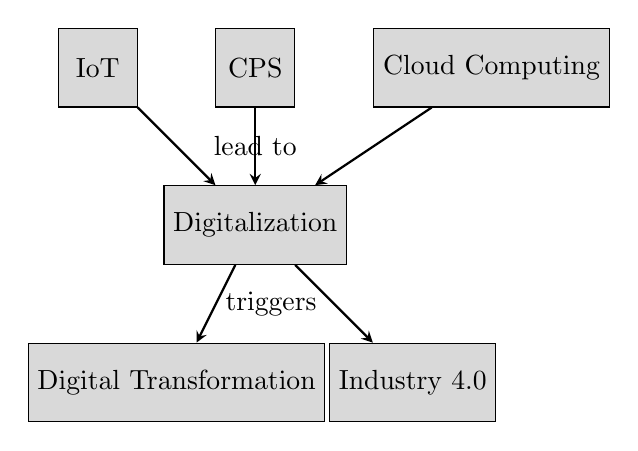
\begin{tikzpicture}[node distance=2cm]

%first row
\node (IoT) [process] {IoT};
\node (CPS) [process, right of=IoT, xshift=0cm] {CPS};
\node (CC) [process, right of=CPS, xshift=1cm] {Cloud Computing};
%second,third row
\node (D) [process, below of=CPS] {Digitalization};
\node (DT) [process, below of=D, xshift=-1cm] {Digital Transformation};
\node (I40) [process, right of=DT, xshift=1cm] {Industry 4.0};

%arrows
\draw [arrow] (IoT) -- (D);
\draw [arrow] (CPS) -- node {lead to}  (D);
\draw [arrow] (CC) -- (D);
\draw [arrow] (D) -- node [xshift=0.7cm]{triggers}(DT);
\draw [arrow] (D) -- (I40);


\end{tikzpicture}
\caption{Relation between terms} \label{fig:terms}
\end{figure}

%JO
%TODO 1) Framework als Begriff klarstellen? 2) Maturity Model mit aufnehmen sobald wir dieses festgelegt haben
%present			%2.1 Terminology
\section{State of digitalization}
We suggest a model to challenge a business to rate itself regarding its "state of digitalization". Companies should objectively rate themselves using their current state and their goal state as a scale and then compare themselves with competitors to create a benchmark. This can describe their current standing in the market and show which components the business already succeeded on and which it needs to focus its attention on. As an example, companies with little previous activity and a low grade of digitalization will start developing a business model and an overall market overview to define their targets while companies that already developed a strategy will skip this step to immediately develop their implementation strategy. With this pattern, a company can develop an individualised strategy based on their industry as well as their individual circumstances.

%To develop a strategy for responding to the impeding changes accompanying \ac{I4.0}, a business should first investigate what components this strategy is composed of.
We suggest to consider three key aspects as core challenges for succeeding during the \ac{DT} which are an adapted form of the four core aspects suggested by the \ac{WEF} \cite{worldforumdigitalenterprise:2016}:
%While the goal of an \ac{I4.0} strategy is apparent, as it is usually congruent with the general economic goals of the business itself, the implementation of this goal is dependent on three fields. 

%We expect everyone to be familiar with the topic of digital transformation so we will refrain from describing estimates of future economic values that range from several hundred billion to a few trillion dollars total. %TODO citation
%We also assume most readers have heard the terms Internet of Things, Industry 4.0 or digital transformation. The argument for why businesses need to carefully evaluate how they implement their strategy and why they execute certain activities can be split into three categories:

\subsection{Technology and operations}
The concept of digital transformation suggests that the entire business goes digital. It also implies that companies will have to adapt to a range of new technologies %TODO cite world http://reports.weforum.org/digital-transformation-of-industries/an-introduction-to-the-digital-transformation-of-industries-initiative/
 each of them potentially affecting an organizations core business. These technologies are not yet standardized nor established and some might be considered obsolete again in the near future. While businesses need to innovate to ensure they differentiate from their competitors, %source lecture Schrader? 
 they also need a stable core business to reduce risks. Open standards and technologies that have been widely accepted can offer these securities.
 % Instead of evaluating all these things by themselves, businesses should look towards existing organizations in the form of industry consortia and other non-profit structures to follow their guideline. By doing this, businesses can
The business also needs to improve its operational performance, using technology to both improve savings and enable new models and answer disruptive competitors \cite[p.15ff.]{worldforumdigitalenterprise:2016}.

%technology

\subsection{Business Models}
A popular term, disruption, describes what technology innovation does to markets. A new technology can lead to a complete overhaul of existing markets and it is usually accompanied by a different business model that catches existing market players off guard \cite{LucasJr200946}. \citeauthor{gassmann2013geschaeftsmodelle} suggest that a core challenge for businesses it not only to be a technological leader but also to develop a new business model that challenges existing market participants and helps a business to differentiate its product from the rest. A common issue for successful businesses is the \emph{Innovator's dilemma}. Businesses need to be willing to disrupt even themselves in order to compete \cite{christensen1997innovator, worldforumdigitalenterprise:2016}.

\subsection{Culture}
\citeauthor{hammer:2015, LucasJr200946} argue a core task of preparation is the adaptation of the organizational culture to enable openness to innovation and adaption to new market environments. Businesses need to be "results-oriented", allow their employees to have the "freedom to increase innovation"\cite{hammer:2015} and avoid a culture that "promotes hierarchy and maintain[s] the status quo [because it] will be resistant to disruptive technologies"\cite{LucasJr200946}.
%business models
%culture
%disruption 				    %4. components digital strategy
\subsection{Frameworks}
\label{subsec:frameworks}


%1. I40 and IIC definition
%2. koloss industries clustering 
%3. what statistcs do we base our categorisation on
%4. where do you see yourself model (aka early adopter etc)

Both the industry and the academic world offer a variety of frameworks, concepts, consulting services and guidelines for businesses, institutions and even cities to employ to optimize their utility from the Digital Transformation.
We focused our attention on frameworks that are applicable to a variety of sections to ensure we define recommendations applicable to businesses independent of region, industry or size. 
We chose four frameworks as applicable to most industries and want to summarize them in the following chapter.

\subsubsection{Industrie 4.0}
The German Industrie 4.0 initiative was created by the German government to improve Germany's economical position in the global market. According to the \emph{Plattform Industrie 4.0}, I4.0 is a specialization of the \emph{Internet of Things and Services} and applies to a subset of all industries, mainly focused on industrial production and manufacturing
\cite[p.41]{umsetzungsstrategie:2015}. Although it is specifically focused on the manufacturing section, it is the most comprehensive initiative we found involving BITKOM e.V., VDMA e.V. and ZVEI e.V., three industrial associations representing IT, electronics and digital economy in Germany \cite{zveimembers:2016, vdmamembers:2016, bitkommembers:2016}. The initiative offers both recommendations and best practices for individual organizations \cite[p.40ff.]{umsetzungsstrategie:2015} as well as describing the strategic plan of progressing the \ac{I4.0} on a national level for the German government \cite[p.15ff.]{umsetzungsstrategie:2015}. It therefore offers a wide range of both high level overviews all the way do very detailed implementation advise on the factory floor.
 The following list summarizes the core goals \cite[p.8]{umsetzungsstrategie:2015}. \footnote{It should be noted that only some of these goals are relevant to individual businesses trying to improve their strategy while others are global environmental necessities. Those that require action of individual businesses are marked with an (X).}

\begin{itemize}
	\item  Standardization (X)
	\item  Reducing of complexity (X)
	\item  Wide band infrastructure
	\item  Security (X)
	\item  Work culture and organization (X)
	\item  Education
	\item  Legal constraints (X)
	\item  Efficiency (X)
\end{itemize}
\footnote{The communication infrastructure as well as education have been excluded under the assumption that they are inputs that are typically not produced by a business itself but rather acquired externally.}

The I4.0 initiative offers several artifacts to support organizations in the transition to a digitalized organization as well as to facilitate the coordination between organizations and industries in researching and developing standards and technologies. 

The most prominent framework is the \ac{RAMI} which has been created as a guideline to avoid definition of multiple, redundant and conflicting standards and communication strategies \cite[p. 41]{umsetzungsstrategie:2015}.

\begin{figure}[H]
\centering
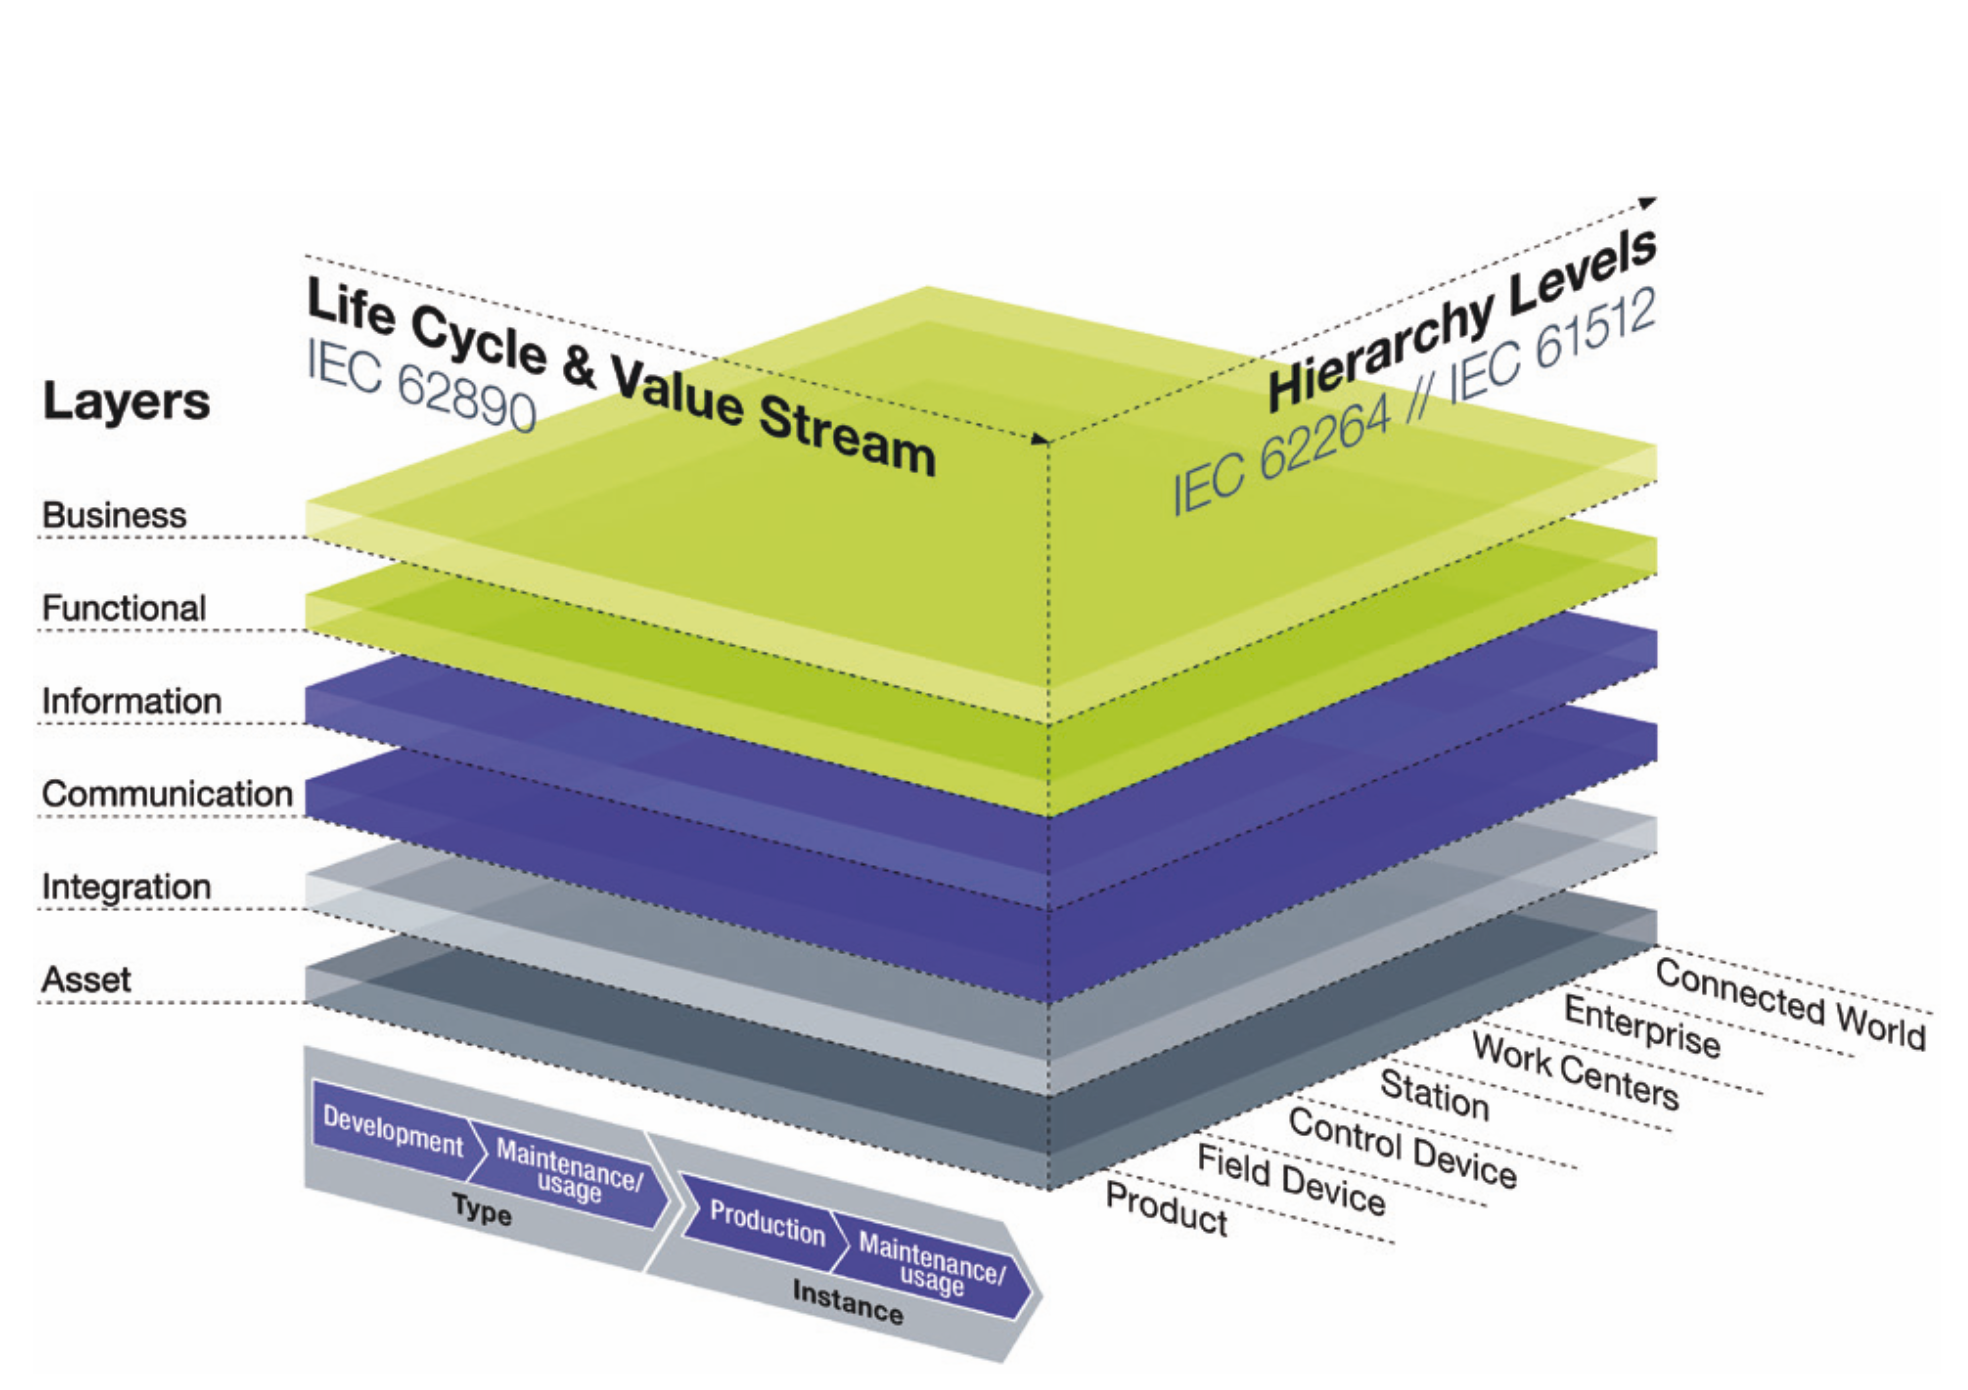
\includegraphics[width=1\columnwidth]{images/RAMI}
\caption{\ac{RAMI} from \citeauthor{umsetzungsstrategie:2015}}
\end{figure}

The \ac{RAMI} framework focuses on three dimensions \emph{layers, Life Cycle \& Value Stream} and \emph{Hierarchy Levels}. By layers, the framework takes reference do different layers of abstraction from a system engineering perspective \cite{Hankel:2015}. 
%three dimensions of RAMI
The "Layers" described are typical IT abstraction for reducing complexity in large systems with numerous components. 
The "Life Cycle \& Value Stream" dimension describes the phases a product goes through from the initial idea and development to the final production and usage. It is compliant to IEC 62890, a governance standard for life cycle management of products.
The "Hierarchy Levels" are referencing to IEC 62264, the international norm for the integration of enterprise IT and control systems in manufacturing. It has been extended with two additional levels, "Product" and "Connected World" to adequately represent the environment of \ac{I4.0} environments \cite{Hankel:2015}.


\subsubsection{Industrial Internet Consortium}
The IIC is an \emph{"open membership organization with 250 members from 30 countries, formed to accelerate the development, adoption and widespread use of interconnected machines and devices, intelligent analytics, and people at work"}\cite{iic-progress:2016}. Its goals are as follows \cite{iic-aboutus:2016}:

\begin{itemize}
	\item  Creation of use cases and testbeds
\item  Develop reference architectures and frameworks
\item  Influence the global development standards process
\item  Facilitate open forums
\item  Build confidence around approaches to security.
\end{itemize}


\subsubsection{Integrating IIC and I4.0}

Both the \ac{IIC} and the \ac{I4.0Init} have announced collaboration efforts to ensure their goal of common standards and structures is achievable. While the IIC's efforts are targeted at a higher level of abstraction, the \ac{I4.0Init}'s focus is more narrow, focusing on the manufacturing and production sections. 


\begin{itemize}
	\item Business Model verification and redesign \cite{gassmann:gallen:2013geschaeftsmodelle}
	\item Organizational Culture
	\item Technological capabilities and expertise
\end{itemize}

\subsubsection{St. Gallen Business Model Navigator}

Since both previous models, the  \ac{I4.0Init} and  the \ac{IIC} primarily address the \emph{technology and operations} dimensions of a digital strategy, the \ac{BMN} is a great resource to help companies evaluate their own and their competitors business models. It focuses on the business model of a company, suggesting that a company can not rely on its products quality and performance alone to succeed but that companies must also reevaluate their business model and those of their competitors. Figure \ref{fig:BMN} shows the 4 dimensions the framework focuses on. Alongside the concept, 55 existing business model types are added that have been inspired by businesses and products of the past. The idea is to reevaluate a businesses own products and capabilities and confront them with various other business models to see new ways of engaging customers and increase profits. Examples of patterns are \emph{Open Source}, \emph{Pay what you want}, \emph{Razor and Blade} or \emph{Robin Hood} \cite{gassmann:gallen:2013geschaeftsmodelle}.

\begin{figure}[H]
\centering
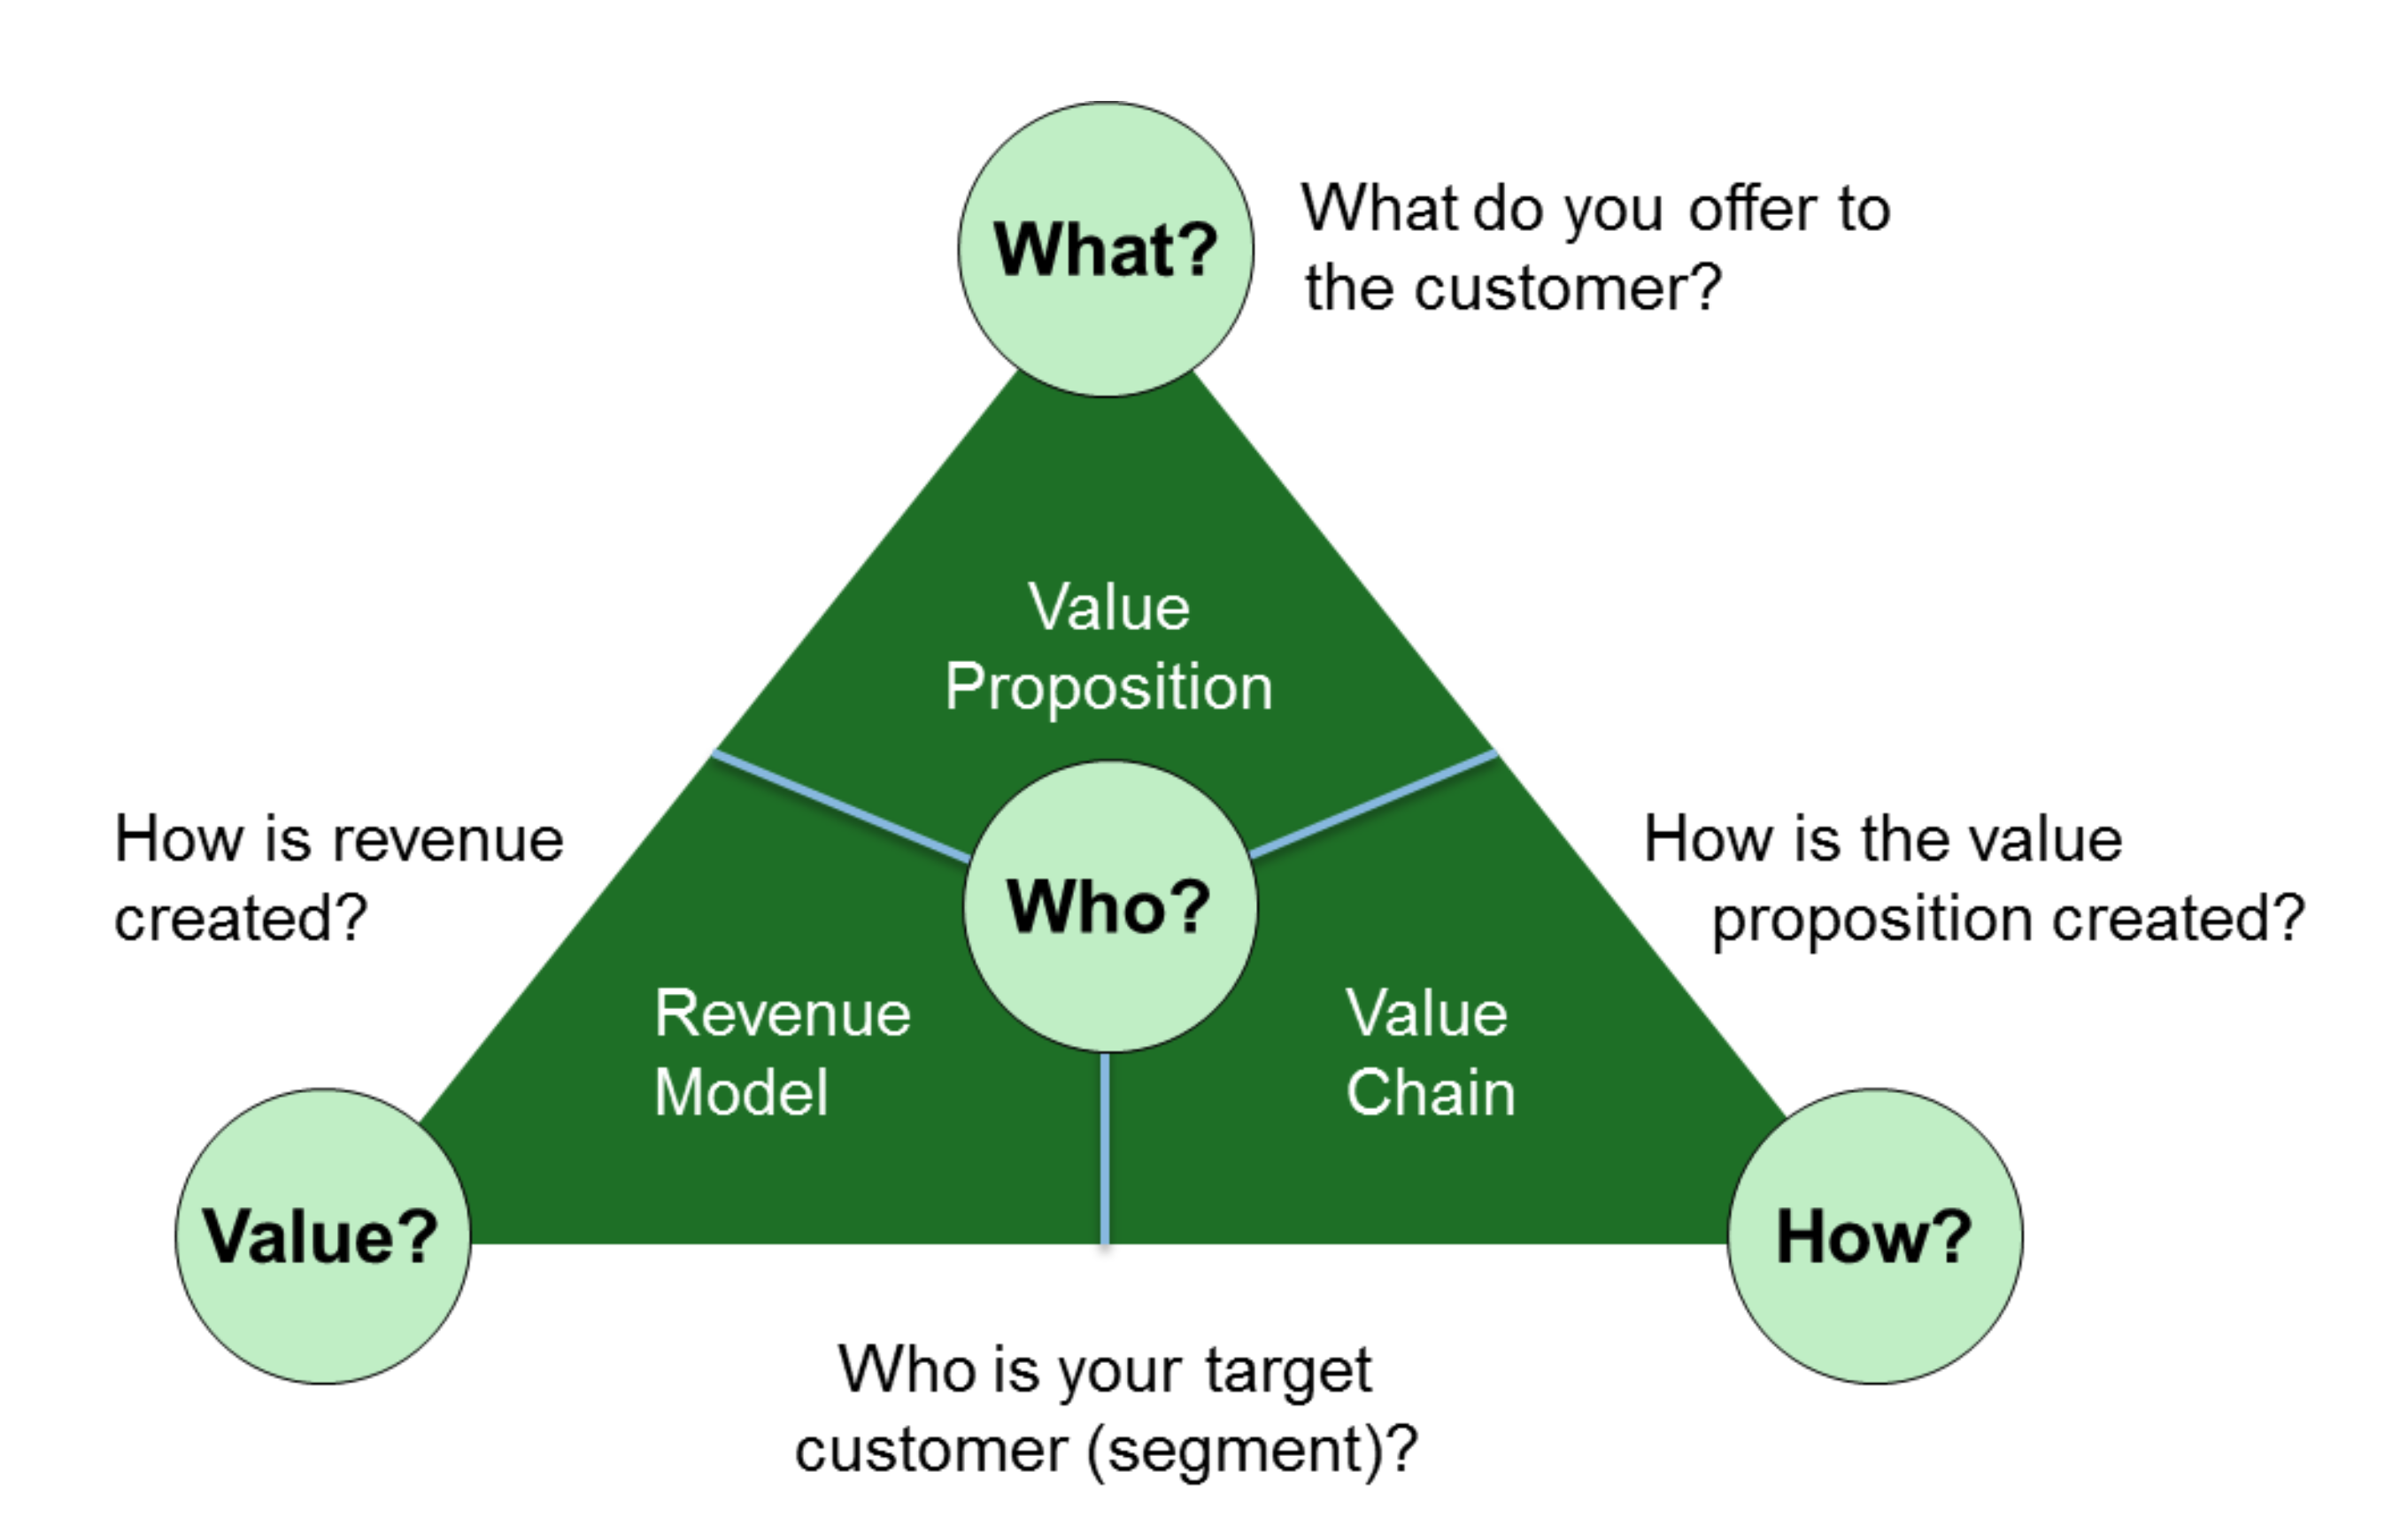
\includegraphics[width=1\columnwidth]{images/BMN}
\caption{Business Model definition - the magic triangle from \citeauthor{gassmann:gallen:2013geschaeftsmodelle}}
\label{fig:BMN}
\end{figure}

%TODO PB St Gallen und MIT Buch einfügen

\subsubsection{Leading Digital}

Technology, operations and business model have been covered, but a business is also strongly influenced by its culture which in turn is strongly influenced by its leadership. While the \ac{WEF} recommends adapting a business culture and focusing on \emph{"attracting and retaining talent in the digital age"}\cite{worldforumdigitalenterprise:2016}, it focuses on attracting millennials and developing the workforce from a human resources perspective. During our literature research we found surprisingly little on the development of corporate culture in regards to \ac{I4.0} and \ac{DT}. \citeauthor{hammer:2015} performed a number of interviews, collecting recommendations by industry experts with an average of 17 years of work experience, summarising the responses with recommendations for more \emph{"trial \& error environments, more employee freedoms, less hierarchy and a two-world IT"}. \citeauthor{bonnect2014leading} encourage a top down approach for shaping a companies culture by communicating goals clearly and often, have the management lead the way in the digital engagement, find digital champions in an organization and amplify their network impact and finally identify quick wins to affirm the strategy of transformation by showing results fast. 


%\subsection{Terminology}

%\begin{itemize}
%\item
%what is Industrie 4.0 in relation to other words in the english-speaking environment
%\item
%does Industrie 4.0 also apply to industries that aren't involved in manufacturing
%\end{itemize}

%Compare to
%\cite{Wirtschaft_en:2016}
%and \cite{Wirtschaft:2016}
%for how the official translation handles the terms
%present 			%2.2 frameworks
 					%5. background
\input{branchcentricdigitalization} %6. branch-centric digitalization
\input{Diffusionofinnovationmodel}	%7. duffusion of innovation model
\section{Individual I4.0 Maturity Model}

To enable an individual \ac{I4.0} strategy and applicable guidance, the section-specific frameworks and emphases provide for relevant information and progress in the respective section. One key element is missing to make this orientation lead to an individual strategy to get \ac{I4.0} processes implemented in the organization of the reader of this paper: The competitive environment or rather the benchmark against others in this specific industry combined with the individual state of digitalization. To solve this, we collated insights to outline the individual maturity model. The objective is to receive an individual scheme on a strategic level, industry-specific and connected to the status quo of the considered organization \& competition, to implement relevant and effective \ac{I4.0} processes and ultimately transform to sustainable solutions.

The following maturity model insights are the basis for the \ac{II4.0MM}, but are either only focusing on manufacturing-specific \ac{I4.0} or not aggregating all relevant data

\begin{enumerate}
\item Industry 4.0 Maturity Model \cite{Schumacher2016161}
\item The Connected Enterprise Maturity Model \cite{RockWellAutomation-connectedEnterpriseMaturityModel}
\item The Digital Advantage: How digital Leaders outperform their peers in every industry \cite{CapgeminiMaturityModelDigitalAdvantage}
\end{enumerate}

The \ac{II4.0MM} is structured into 3 steps, which are described subsequently, enriched with the appropriate frameworks and studies.


\begin{figure}[H]
\centering
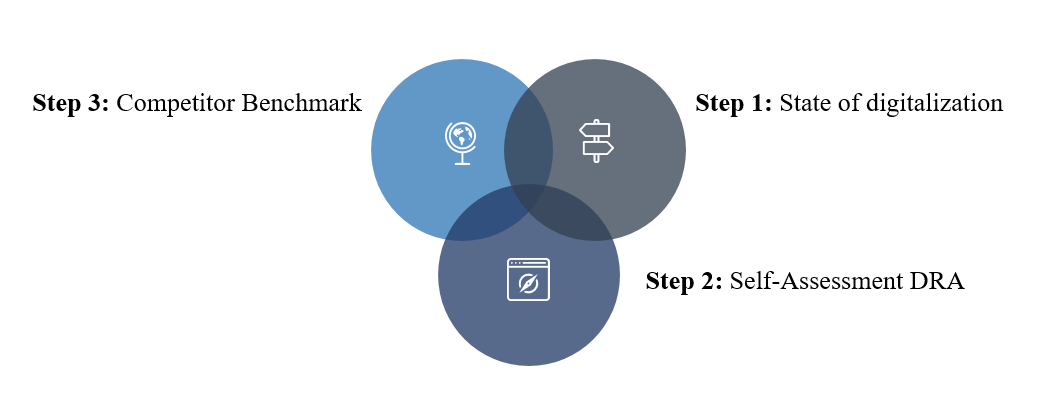
\includegraphics[width=1\columnwidth]{images/II40MM_grafik.PNG}
\caption{\ac{II4.0MM} 3 steps: State of digitalization, Self-Assessment (DRA), Competitor Benchmark}
\end{figure}

It is important to define what is meant with the term \emph{\ac{II4.0MM}}. In this paper, we combine the three key aspects of the state of digitalization, which are described in chapter \emph{2.2} %TODO kann man das hier irgendwie noch besser darstellen mit der Referenz zum vorherigen Kapitel im Paper? %
with self-assessment tools to get the benchmark of the competition in the considered industry to shape an applicable model. This can be used to get strategic leaders converted to implement digital and \ac{IoT} processes in their respective organization.
Other studies may call it \emph{digital Readiness}, which is not focusing on \ac{I4.0} or \ac{DT} in detail.

The first step of the \ac{II4.0MM} is to determine the state of digitalization. A quick hint is delivered by the four Types of Digital Maturity by \cite[p.4]{CapgeminiMaturityModelDigitalAdvantage}:

\begin{figure}[H]
\centering
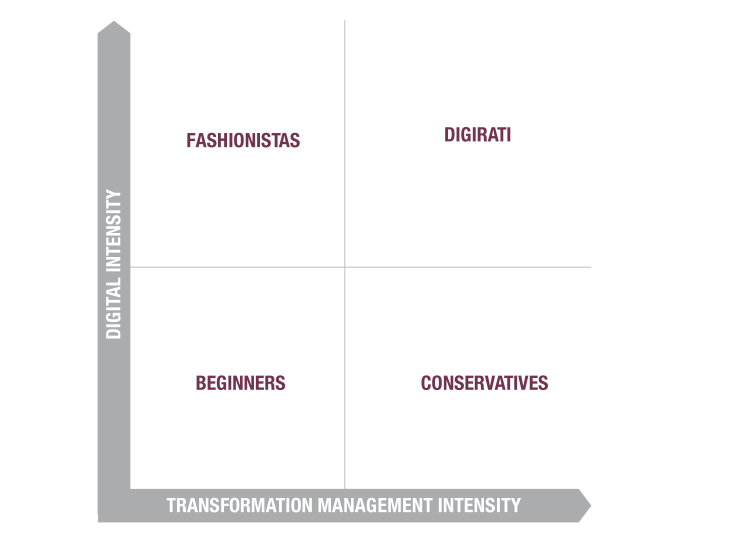
\includegraphics[width=1\columnwidth]{images/maturityModel_4segments_capgemini.PNG}
\caption{Four Types of Digital Maturity: Fashionistas, Digirati, Beginners, Conservatives \cite{CapgeminiMaturityModelDigitalAdvantage}}
\end{figure}

Those four types are distinguished by the affiliation to two dimensions: digital intensity (technology-enabled initiatives) and transformation management intensity (leadership capability) \cite{CapgeminiMaturityModelDigitalAdvantage}. Extending those dimensions with the business models as the third key aspects of the state of digitalization, we can see an analogy to our predefined model.

Every organization can classify themselves into one described type by answering specific questionnaires or deploy a \ac{DRA} \cite{Schumacher2016161} \cite{ReadinessIndustrie40Impulse} \cite{i40-self-assessment-PwC:2016}. After the first segmentation it is recommended to establish a connection to individual competition benchmark. This is the second step of the \ac{II4.0MM}. General information can be found in our chapter 3 \emph{Sector specific application of frameworks} and the respective recommended frameworks with further information. The \ac{II4.0MM} cannot deliver further benchmark information but the urgency of transformation can be explorated via the following resources:
\begin{enumerate}
\item Digital Readiness Assessment: Does your business strategy work in a digital world? \cite{ey-dra}
\item IMPULS – Industrie 4.0 Readiness \cite{ReadinessIndustrie40Impulse}
\item Industry 4.0 Self Assessment \cite{i40-self-assessment-PwC:2016}
\end{enumerate}

This step concludes the \ac{II4.0MM} and delivers a scheme, which can be used for \ac{I4.0} implementation in the individual context.
 			%8 Individual Digi strategy
\section{Conclusion}

In this paper, we provide a systematic approach to make industry 4.0 strategies, concepts and processes applicable in selected \ac{ISIC}-aggregated sections. The opportunities of the implementation of those measures are depending on business characteristics, the state of digitalization and ultimately the individual \ac{I4.0} maturity. We found, that \ac{I4.0} frameworks are mainly focusing on one core industry: \emph{Manufacturing}. Therefore, insights of that specific industry may not be applicable in other industries with appreciably different business environment and attributes. Nevertheless, reference models like the \ac{RAMI} and guidelines of the \ac{IIC} are building keystones for every industry and can be used for the digital strategy derivation with appropriate transferring of concepts to the actual business and its environment. Extending this with the \ac{II4.0MM}, organizations can get profound insights and convertible concepts how they can implement \ac{I4.0} in their respective environment and context.

As this \emph{revolution} touches a lot of business areas and interrelations, \ac{I4.0} is a macroeconomic phenomenon which affects whole business models and markets, as well as extensive strategic decisions. It is important to get a holistic insight to arrange profound decision-making.

One result of this paper, the \ac{II4.0MM}, is limited to be used as a systematic approach to develop strategic schemes and the perception of change in one specific section or organization itself. Another limitation of this paper is anchored in the holistic review of section-specific literature and frameworks. Therefore, in opposite of detailed information in one specific industry the overview on every \ac{ISIC} section is preferred. This approach limits the in-depth insight of the application of frameworks in one respective section.

To develop tangible action plans we recommend further investigation and research, as well as professional consulting, innovation management or interim management. The interconnection between industries and different business models requires technical standards and cultural change in organizations. Several frameworks can be used to implement \ac{I4.0} measures, individually fitted to the respective business environment. Nevertheless, it is important to state out, that the basis of change and transformation can only be provided by the culture or rather the leadership of organizations. The review of several studies show, that it is important to conduct more studies which recommended actions after defining the \ac{I4.0} maturity level or digital readiness combined with the comparison with competitors or new evolving business models. A study, which investigates a bridge between the \ac{II4.0MM} and reliable data of competitors in the respective industry or even the recommendation of cooperation partners, who can leverage the progress of individual \ac{I4.0} implementation, would fill the gap of knowledge stated out in this paper.

Some industries are facing an urgent demand for action and others can gradually develop new concepts for the respective change management. This paper shows, that many industries are being confronted by changes, challenges and chances by the impacts of \ac{I4.0} and need holistic strategies to build sustainable solutions.




%\section*{Acknowledgments}


\begingroup
\def\UrlBreaks{\do\/\do-}
\bibliographystyle{IEEEtranN}
\bibliography{references}
\endgroup
\end{document}
